\documentclass{article}

\usepackage{graphicx,float}
\usepackage{hyperref}

% Title content
\title{\Large KEN 4154 Assignment 3 \\ \normalsize Reinforcement Learning}
\author{Adrian Sondermann, Abel de Wit}
\date{November 24, 2020}

\begin{document}

\maketitle

\section{Introduction}
In this assignment we were tasked to implement a type of reinforcement learning with the OpenAI testbed 'Mountain Car'. In this environment, the car is tasked to drive on a sinus function and its goal is to reach the top of the hill. For most people this task seems trivial; Go back and forth between the two hills to build up some momentum and then use that to reach the top of the hill. This however, is less intuitive for algorithms as driving up the left hill would mean removing the car further from the goal. Because of this, regular pathfinding algorithms will have difficulty with distancing themselves from the goal first, to then be able to reach the goal. 

To solve this, the problem is reformulated to be used by reinforcement learning. Using reinforcement learning, the algorithm can learn what the reward will be in a situation if taken a certain action, these are called state-action pairs. 

\section{Implementation}
\subsection{Environment}
Using the \texttt{gym} package provided by OpenAI the environment is set up rather easy. 
The environment provides us with several things:
\subsubsection{Observation}
The observation describes the current state of the environment. 
In the case of our 'Mountain Car' example we are provided with two values. 

The first is the horizontal position of the car in the environment. This value ranges from $-1.2$ to $0.6$. The car starts in a random position between -0.6 and -0.4, which is the valley in our environment. 

The second value of the observation is the speed of the car. This value ranges from -0.07 to 0.07, where a negative value indicates moving to the left and a positive value indicates moving to the right.

\subsubsection{Step function}
The environment has a function called step. This function takes as a parameter the action that is to be taken, and outputs four values. The observation (state) after taking the action, the reward of this action, whether the objective is reached '\texttt{done}', and some information which is irrelevant for our scenario. 

\subsubsection{Discretising state space}
As Q-learning requires a discrete state space, both variables, speed and position were partitioned into equal-width bins. The speed of the car was rounded to 2 decimal digits, its position to 1 decimal digits. Thus the state space consits of $15 \cdot 19 = 285$ states.

\subsection{Q-learning}
Using the environment described above, we were able to implement a very basic Q-learning algorithm that is able to teach itself what types of actions should be taken in which states. 
It teaches itself this trough repeated trial and error, these trials are called \texttt{episodes}. For each episode the environment is reset and a certain set of actions are taken by the algorithm. 

The Q-learning algorithm uses epsilon greedy\footnote{\url{https://www.geeksforgeeks.org/epsilon-greedy-algorithm-in-reinforcement-learning/} } (see Figure \ref{fig:epsilon}) to determine whether it will choose an action randomly or based on the learned Q-function. The epsilon is lowered while learning to slowly force the algorithm to use the Q-function more than random moves, but these random moves are what makes the algorithm go to unexpected states which increases the learning of the environment. 

\begin{figure}[h!]
    \centering
    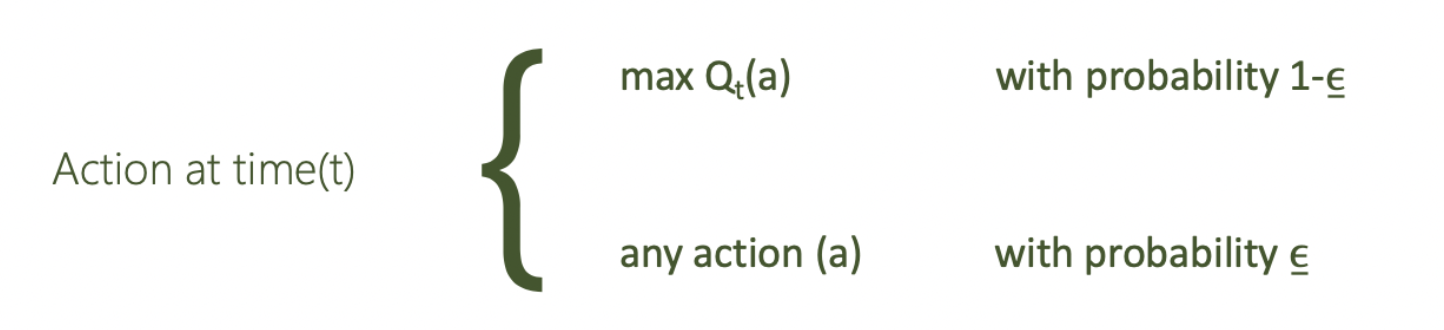
\includegraphics[width=0.75\textwidth]{Epsilon_greedy.png}
    \caption{Visualization of the average rewards per episode}
    \label{fig:epsilon}
\end{figure}


After it has chosen an action either randomly or based on the highest value in the Q function for the current state, the step function which is described above is called with the chosen action. The result of taking this action is recorded in the four variables that are returned. The new state is discretised and the Bellmann update is performed on the Q-function. 
\begin{displaymath}
  Q(s, a) = Q(s,a) + \alpha[R(s,a) + \gamma max Q(s', a') - Q(s, a)]
\end{displaymath}

The reward that is achieved by doing action 'a' in state 's' is given by the step function. The new state that we're in '$s'$' is also given by the step function. And with these values we can lookup the Q-values $Q(s, a)$ and $max Q(s', a')$. 
With enough episodes of randomly moving around in the environment, the algorithm starts to reach the goal more and more often, because of this the algorithm will learn a policy of which action is the best to take in a certain state. In the case of our 'Mountain Car' environment, that means that the algorithm learns whether to move left or right given his position on the hills and his current speed.


\section{Results}

\subsection{Visualisation}
To visualize the state-value function $Q$ the maximum per discretisised two-dimensional state (velocity, position) is calculated. Then the retreived 2d-matrix is displayed using the \textit{viridis} colormap.

\subsection{Tuning}
A good visualization of the function must contain information about how the car will behave in different situations, respectively the distance to drive until the destination will be reached. Therefore the parameters in Table \ref{tab:tuned_params} were determined. The big discount rate is useful to gain insight of how far the car has to travel, beginning from its current position and velocity. A small epsilon guarantees few random moves, as these are only initially needed. This is because, the algorithm needs to learn driving away from the destination when climbing the hill slowly. Afterwards, random moves won't be needed. 5000 episodes are enough for the algorithm to converge, as shown by the convergence in Figure \ref{fig:average_rewards}.


\begin{table}
    \centering
    \begin{tabular}{l|c}
        parameter & value \\
        \hline
        learning rate & 0.2 \\
        discount & 0.9999 \\
        epsilon & 0.01 \\
        minimal epsilon & 0 \\
        episodes & 5000 \\
    \end{tabular}
    \caption{Tuned parameters}
    \label{tab:tuned_params}
\end{table}

\begin{figure}
    \centering
    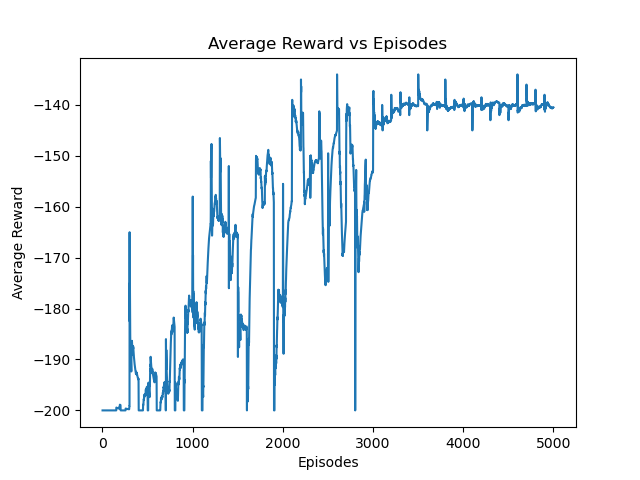
\includegraphics[width=0.75\textwidth]{rewards.png}
    \caption{Visualization of the average rewards per episode}
    \label{fig:average_rewards}
\end{figure}

\begin{figure}
    \centering
    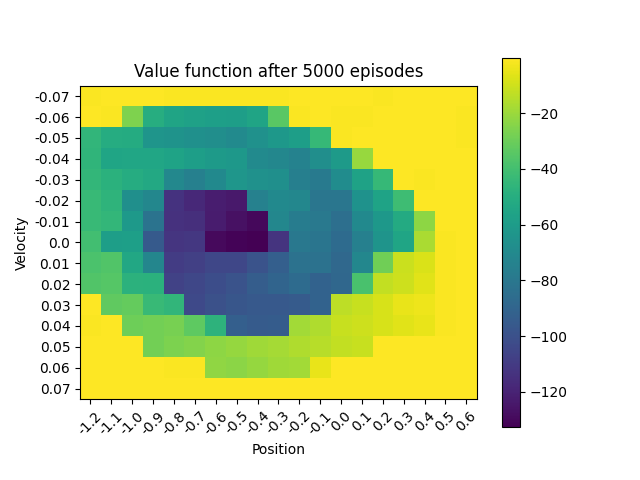
\includegraphics[width=0.75\textwidth]{state-value-function.png}
    \caption{Visualization of the state-value function}
    \label{fig:state-value-function}
\end{figure}

The state-value function in Figure \ref{fig:state-value-function} beautifully visualises the time left the car has to drive before reaching the destination. It starts in the dark middle of the plot without any speed. Initially it needs to gather speed by driving back and forth, until it is fast enough to climb the hill completely. This results in a snake-like shape of the final function. Hence, if the car is fast enough (upper and lower end of the plot) it takes very few timesteps to reach the goal.

\end{document}
